% Не забудьте установить пакет cm-super
%   для использования векторных шрифтов при генерации документа
\documentclass[fleqn, xcolor=x11names]{beamer}

\usepackage{pgfplots}
\pgfplotsset{compat=1.18}
\usetheme{MyAmsterdam} % тема
\usecolortheme{default}

\usepackage[T2A]{fontenc}
\usepackage[utf8]{inputenc}
\usepackage[english,russian]{babel}
\usepackage[bibstyle=gost-numeric]{biblatex}

\usepackage{amsmath}
\usepackage{amsfonts}
\usepackage{amssymb}
\usepackage{hyperref}
\usepackage{graphics, graphicx}
\usepackage{color}
\usepackage{enumerate}

\usepackage{pgfplots}
\usepackage{tikz}
\usetikzlibrary{patterns}

\usepackage{minted}
\usemintedstyle{default}

\usefonttheme[onlymath]{serif}  % привычный шрифт для математических формул

\newminted[pcode]{python}{baselinestretch=1, fontsize=\small}
\newmintinline[pinline]{python3}{baselinestretch=1}
\definecolor{bg}{rgb}{0.95,0.95,0.95}
\newmintinline[linline]{latex}{baselinestretch=1}

\usepackage{tcolorbox}
\tcbuselibrary{minted,skins}

\newtcblisting{lcode}{
    listing engine=minted, %use minted for highlight
    colback=lcodebg, %background color
    colframe=black!50, %width of frame
    listing only,
    minted style=colorful,
    minted language=latex,
    minted options={linenos=false,texcl=true}, %lines - number of lines
    left=1mm,
}
\definecolor{lcodebg}{rgb}{0.95,0.95,0.95}


\usepackage{tikz}
\usetikzlibrary{arrows,positioning}
\usepackage{listings}
\lstset{language=Python}

\newcommand{\real}{\mathbb{R}}
\newcommand{\norm}{\mathop{\rm norm}\limits}
\newcommand{\softmax}{\mathop{\rm softmax}\limits}

\definecolor{beamer@blendedblue}{rgb}{0.037,0.366,0.75}
\defbeamertemplate{footline}{myframe number}
{
  \hfill%
  \usebeamercolor[fg]{page number in head/foot}%
  \usebeamerfont{page number in head/foot}%
  \raisebox{5pt}[0pt][0pt]{% <--- change here
    \insertframenumber\,/\,\inserttotalframenumber\kern1em}%
}
\setbeamertemplate{footline}[myframe number]

\title[Введение в Python]{\bfseries Занятие 5.2: Введение в систему верстки \TeX}
\author[Находнов~М.\,С.]{Находнов Максим Сергеевич}
\subtitle{Практикум на ЭВМ, осень 2022}
\institute[OM]{кафедра ММП, ВМК МГУ}
\date{06 октября 2022 г.}

\graphicspath{{Figures/}} % относительный путь к каталогу с рисунками - чтобы каждый раз не писать
\addbibresource{references_rus_utf8.bib}

\begin{document}

\begin{frame}
    \maketitle
\end{frame}

\section{Система разметки \TeX}
\subsection*{}

\begin{frame}{Система \TeX}
    \TeX~--- система компьютерной вёрстки, построенная по принципу компиляции документа, записанного с помощью специального языка разметки.\\

    Изобретена Дональдом Кнутом в конце 70х годов.\\

    Является де-факто стандартом для написания научных статей.\\

    Язык разметки \TeX\ используется для набора формул во многих системах: в вики-разметке, в matplotlib, Microsoft Office и других\\

    \LaTeX --- надстройка поверх \TeX.
\end{frame}

\begin{frame}{Дистрибутивы и редакторы \TeX}
    Дистрибутивы:
    \begin{itemize}
        \item Windows: MiKTeX, TeX Live
        \item Linux: TeX Live
        \item Mac OS: MacTeX, TeX Live
    \end{itemize}

    \hfill

    Редакторы: WinEdt, TeXnicCenter, Kile, TeXmaker, TeXstudio \ldots
\end{frame}

\begin{frame}{Дистрибутивы и редакторы \TeX}
    Рекомендуемые редакторы:
    \begin{itemize}
        \item VSCode + Latex Workshow. \href{https://youtu.be/DL70VzEqY5Y}{Инструкция по установке}
        \item TeXstudio
        \item Overleaf --- облачный редактор. \href{https://ru.overleaf.com/learn/latex/LaTeX_video_tutorial_for_beginners_(video_1)}{Туториал}
    \end{itemize}
\end{frame}

\begin{frame}{Режимы компиляции}
    \begin{itemize}
        \item \texttt{tex -> dvi -> ps -> pdf}
        \item \texttt{tex -> dvi -> pdf}
        \item \texttt{tex -> pdf}
    \end{itemize}
\end{frame}

\begin{frame}[fragile]{Структура файла .tex}
    \begin{tcolorbox}
        \inputminted[]{latex}{./simple_template/main.tex}
    \end{tcolorbox}
\end{frame}

\begin{frame}[fragile]{Разделы и подразделы}
\begin{lcode}
\section{Раздел 1}
\subsection{Подраздел}
\subsubsection{Подподраздел}

\section{Раздел 2}
\end{lcode}
\end{frame}

\begin{frame}[fragile]{Окружения списков}
\begin{lcode}
\begin{itemize}
    \item Пункт
    \item Ещё один пункт
\end{itemize}
\begin{enumerate}
    \item Пункт 1
    \item Пункт 2
\end{enumerate}
\end{lcode}

    \begin{figure}[h!]
        \begin{minipage}[b]{0.45\textwidth}
            \begin{itemize}
                \item Пункт
                \item Ещё один пункт
            \end{itemize}
        \end{minipage}
        \begin{minipage}[b]{0.45\textwidth}
            \begin{enumerate}
                \item Пункт 1
                \item Пункт 2
            \end{enumerate}
        \end{minipage}
    \end{figure}
\end{frame}

\begin{frame}[fragile]{Формулы}

\begin{lcode}
Формула в тексте: $\sin^2x + \cos^2x = 1$.
\end{lcode}

Формула в тексте: $\sin^2x + \cos^2x = 1$.

\begin{lcode}
Выносная формула:
$$
A_{ij} = b_i^2 + c_j^3\quad \forall i,j=1,\dots,n.
$$
\end{lcode}

Выносная формула:
$$
A_{ij} = b_i^2 + c_j^3\quad \forall i,j=1,\dots,n.
$$

\end{frame}

\begin{frame}[fragile]{Формулы}

\begin{lcode}
Выравнивание по левому краю: \[ x^n + y^n = z^n \]
\end{lcode}

Выравнивание по левому краю: \[ x^n + y^n = z^n \]

\begin{lcode}
    \begin{equation}
        \sin^2x + \cos^2x = 1 \label{eq:trig_eq}
    \end{equation}
    Ссылка по метке: \ref{eq:trig_eq}
\end{lcode}

    \begin{equation}
        \sin^2x + \cos^2x = 1 \label{eq:trig_eq}
    \end{equation}
    Ссылка по метке: \ref{eq:trig_eq}

\end{frame}

\begin{frame}[fragile]{Формулы}
\begin{lcode}
Выравнивание формул:
\begin{align}
\notag p(y|x) = \frac{p(x|y)p(y)}{p(x)} &= \\
\label{eq:bayes}&= \frac{1}{Z}p(x|y)p(y)
\end{align}
\end{lcode}

    Выравнивание формул:
    \begin{align}
    \notag p(y|x) = \frac{p(x|y)p(y)}{p(x)} &= \\
    \label{eq:bayes}&= \frac{1}{Z}p(x|y)p(y)
    \end{align}

\end{frame}

\begin{frame}[fragile]{Ссылки}
\begin{lcode}
\begin{equation}
\label{eq::1}
E = mc^2.
\end{equation}

Ссылка на формулу~\eqref{eq::1}
\end{lcode}
\begin{equation}
\label{eq::1}
E = mc^2.
\end{equation}

Ссылка на формулу~\eqref{eq::1}

\begin{lcode}
\section{Ссылки}\label{sec:1}
Ссылка на раздел~\ref{sec:1} в документе.
\end{lcode}

\end{frame}

\begin{frame}[fragile]{Картинки}
\begin{lcode}
Картинка в тексте:
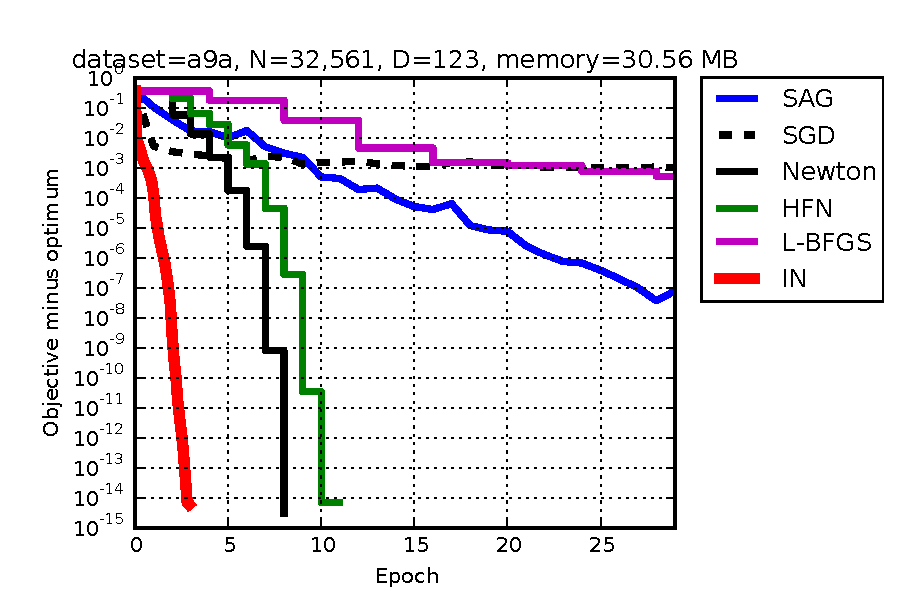
\includegraphics[width=5cm]{a9a_epoch.pdf}
\end{lcode}

Картинка в тексте:
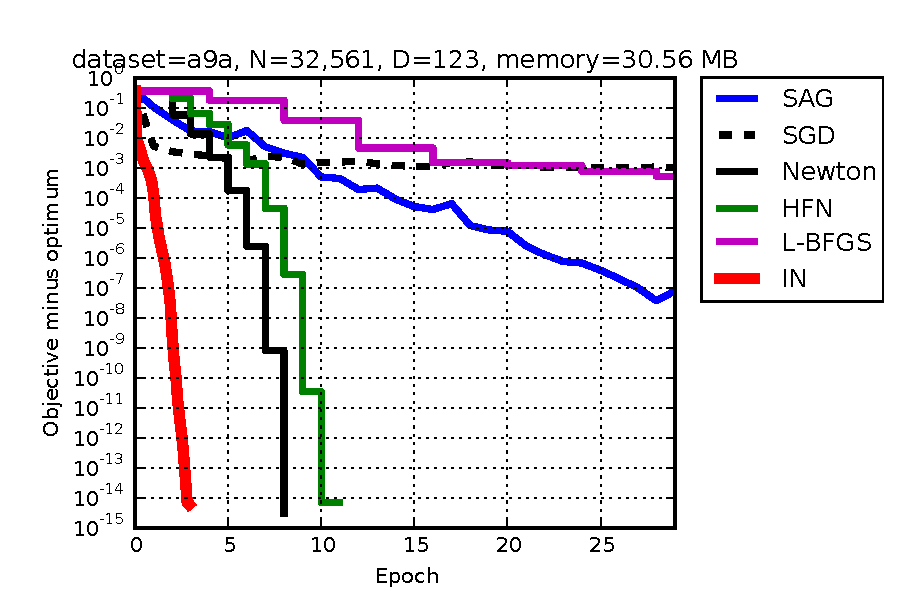
\includegraphics[width=5cm]{a9a_epoch.pdf}
\end{frame}

\begin{frame}[fragile]{Таблица}
\begin{lcode}
Таблица:
\begin{tabular}{|cc|c}
    Column A & Column B & Column C \\
    \hline
    a & b & $\frac{c}{t}$ \\
    d & e & f \\
\end{tabular}
\end{lcode}

    Таблица:
    \begin{tabular}{|cc|c}
        Column A & Column B & Column C \\
        \hline
        a & b & $\frac{c}{t}$ \\
        d & e & f \\
    \end{tabular}

    Существуют \href{https://www.tablesgenerator.com/}{сервисы для автоматической генерации таблиц}.
\end{frame}

\begin{frame}[fragile]{Расположение картинок на странице}

\begin{lcode}
\begin{figure}[h]  %Разместить таблицу здесь
    \begin{center}
        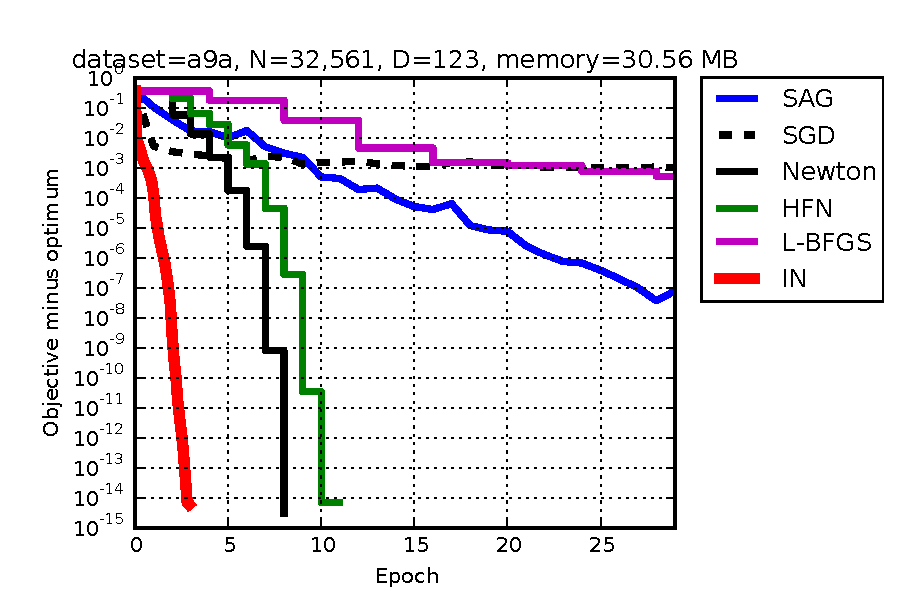
\includegraphics[width=5cm]{a9a_epoch}
    \end{center}
    \caption{Картинка}\label{fig::1}
\end{figure}

Ссылка на картинку: рис.~\ref{fig::1}
\end{lcode}
\end{frame}

\begin{frame}[fragile]{Несколько картинок на странице}
\small
\begin{lcode}
\tabcolsep = 20pt %длина разделителя между колонками
\begin{tabular}{cc}
    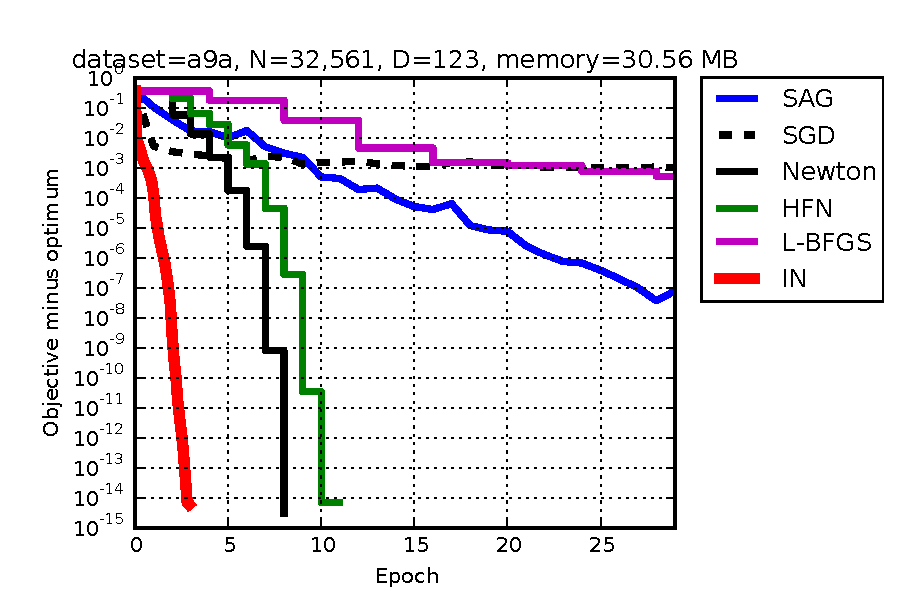
\includegraphics[width=5cm]{a9a_epoch}
    &
    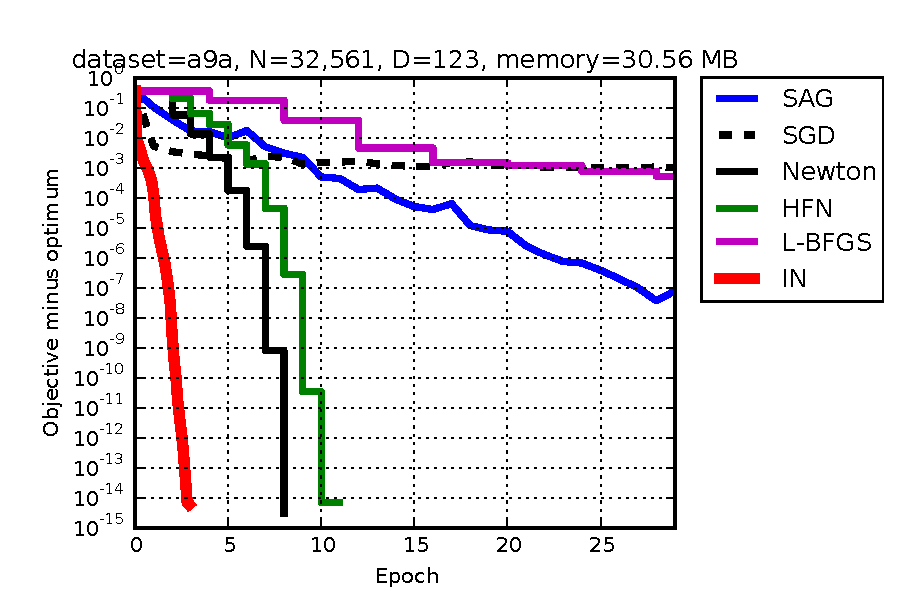
\includegraphics[width=5cm]{a9a_epoch}\\
    (a) & (b)
\end{tabular}
\end{lcode}

    \begin{center}
        \begin{tabular}{cc}
            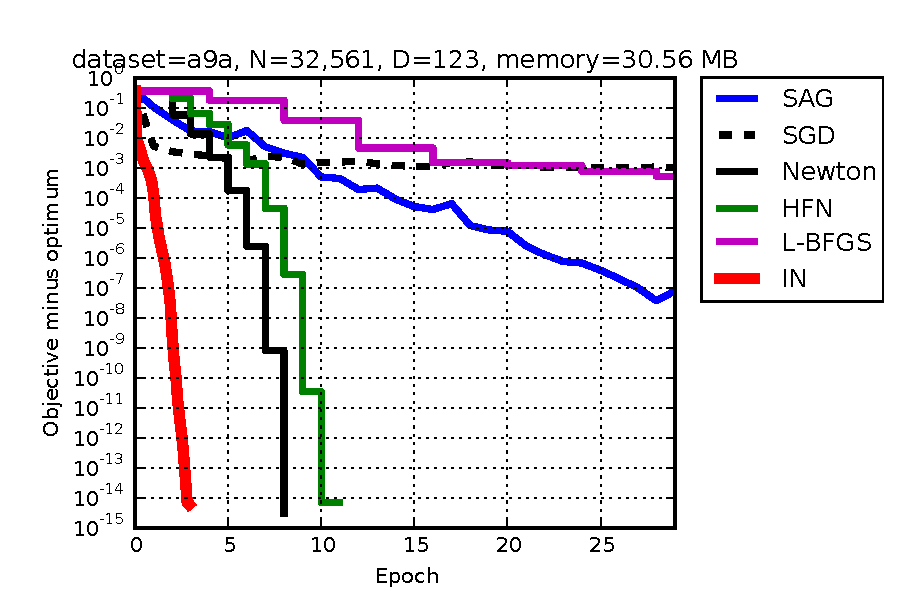
\includegraphics[height=2cm]{a9a_epoch}
            &
            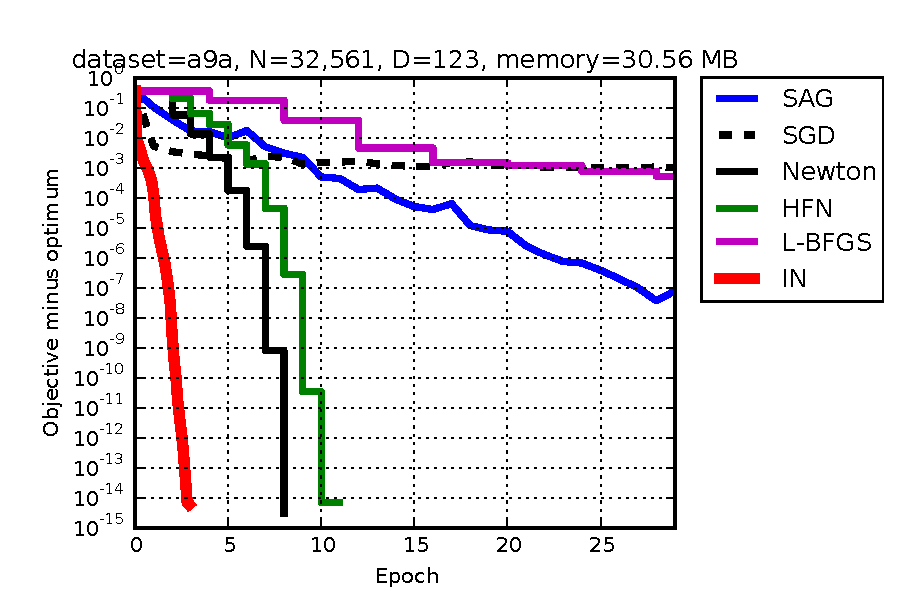
\includegraphics[height=2cm]{a9a_epoch}
            \\
            (a) & (b)
        \end{tabular}
    \end{center}
\end{frame}

\begin{frame}[fragile]{Несколько картинок на странице}
\small
\begin{lcode}
\begin{figure}[h]
    \begin{minipage}[b]{0.45\textwidth}\centering
        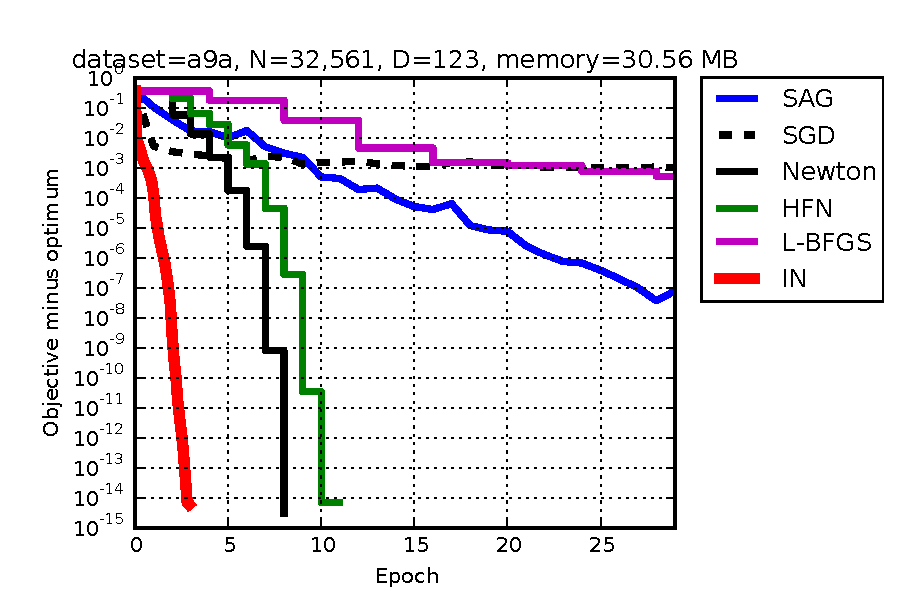
\includegraphics[height=2cm]{a9a_epoch}
    \end{minipage}
    \begin{minipage}[b]{0.45\textwidth}\centering
        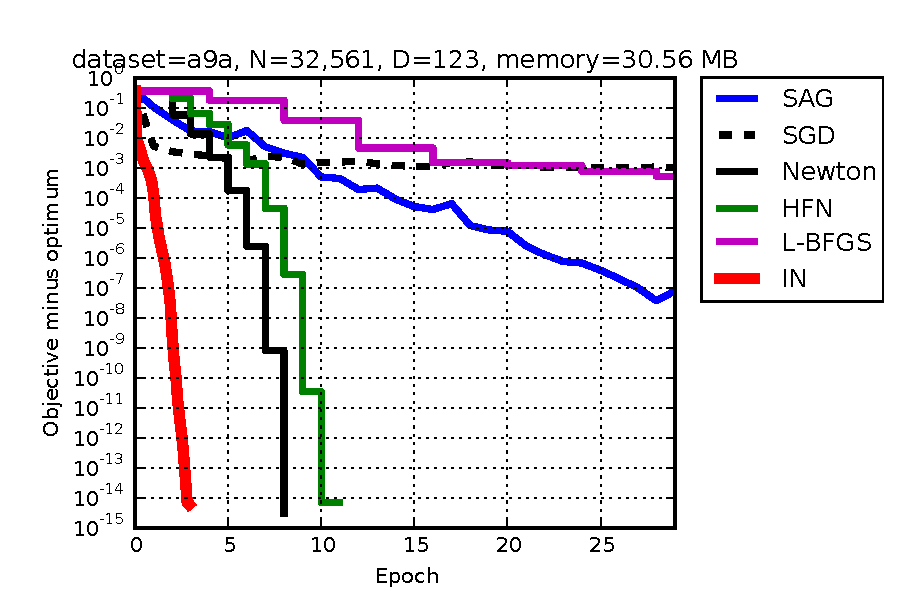
\includegraphics[height=2cm]{a9a_epoch}
    \end{minipage}
\end{figure}
\end{lcode}

    \begin{figure}[h]
        \begin{minipage}[b]{0.45\textwidth}\centering
            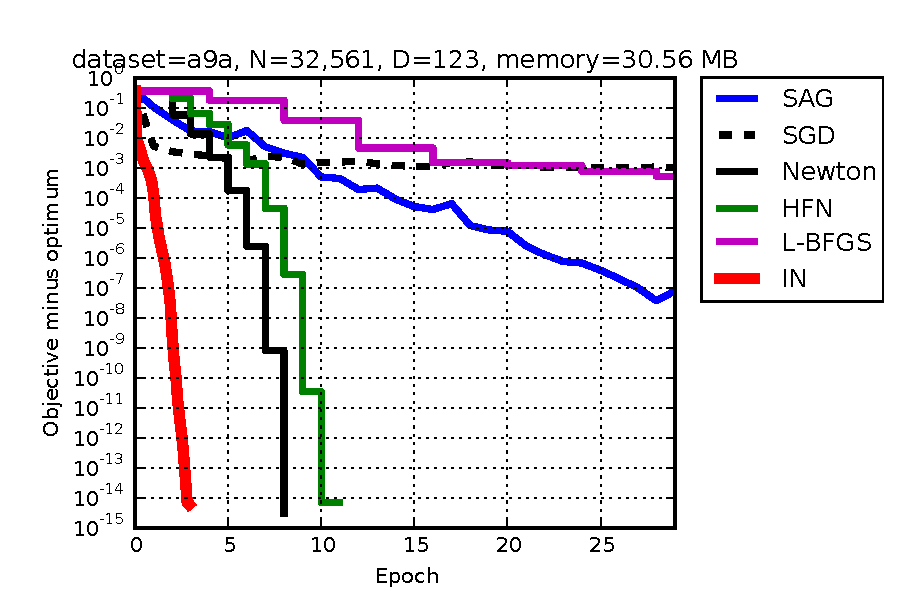
\includegraphics[height=2cm]{a9a_epoch}
        \end{minipage}
        \begin{minipage}[b]{0.45\textwidth}\centering
            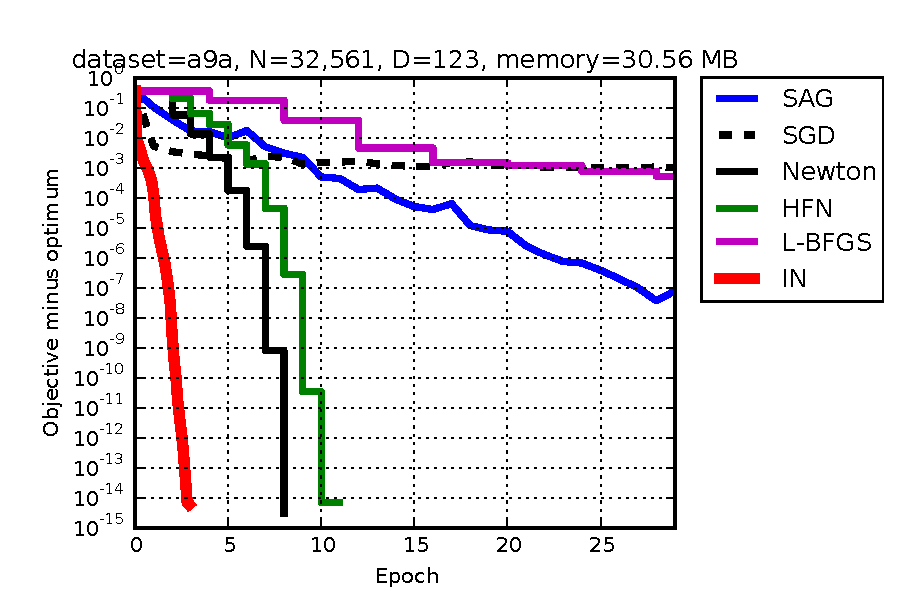
\includegraphics[height=2cm]{a9a_epoch}
        \end{minipage}
    \end{figure}
\end{frame}

\begin{frame}[fragile]{Управление отступами на странице}
    \begin{figure}[h]
        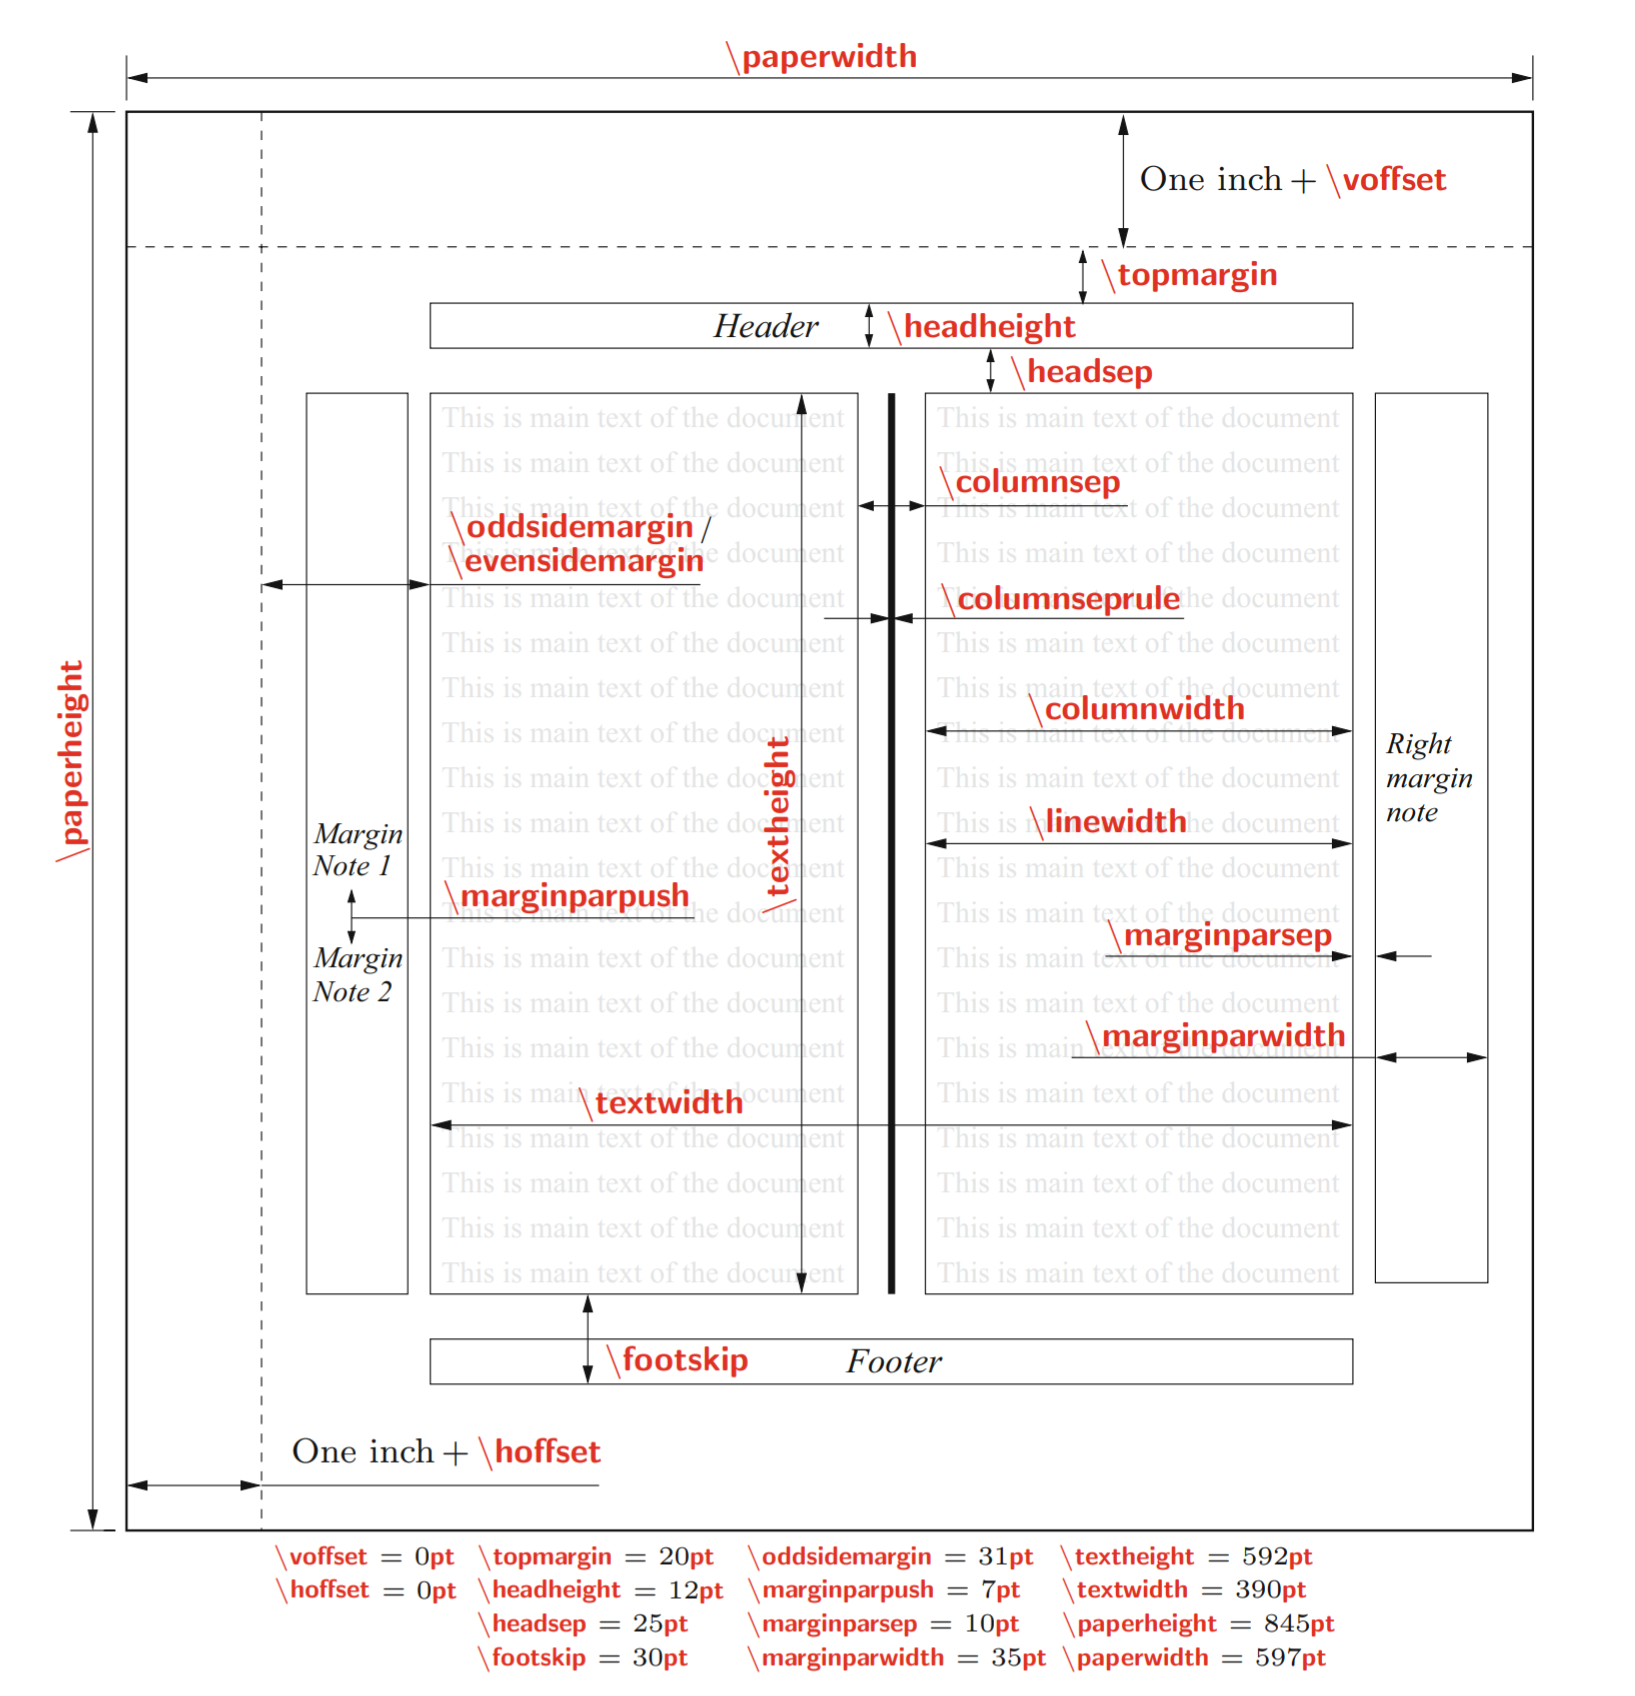
\includegraphics[height=7cm]{Layout.png}
    \end{figure}
\end{frame}

\begin{frame}[fragile]{Несколько команд для управлением текстом}
    \begin{figure}[h]
        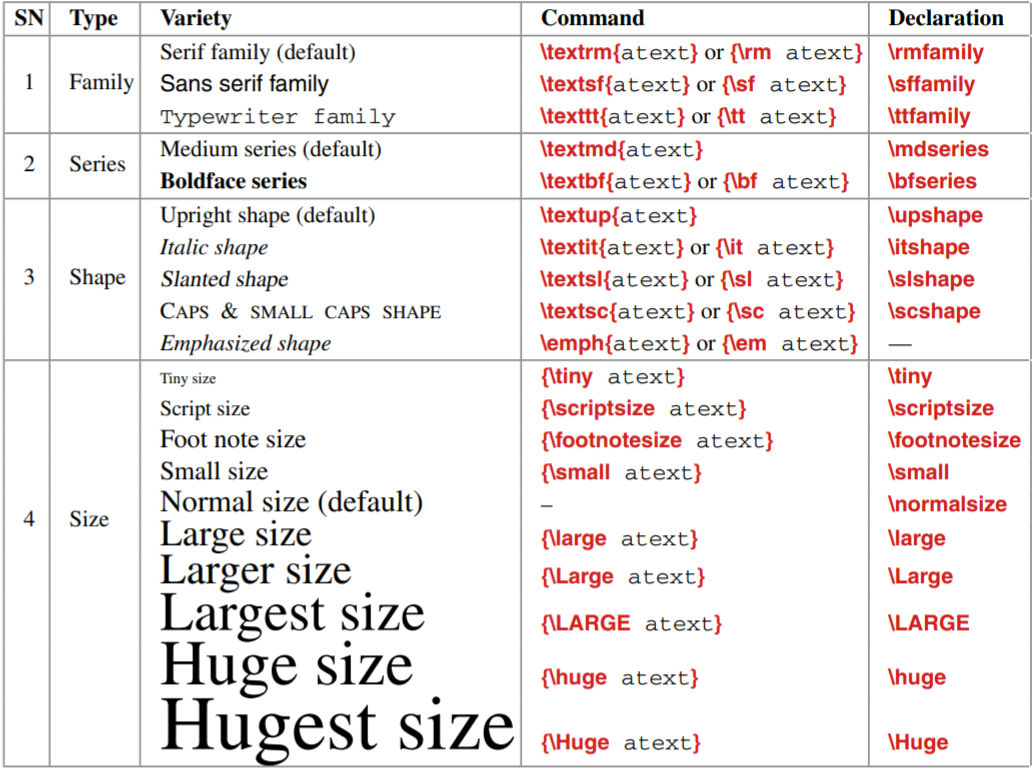
\includegraphics[height=7cm]{Fonts.png}
    \end{figure}
\end{frame}

\begin{frame}[fragile]{Несколько команд для управлением текстом}
    \begin{figure}[h]
        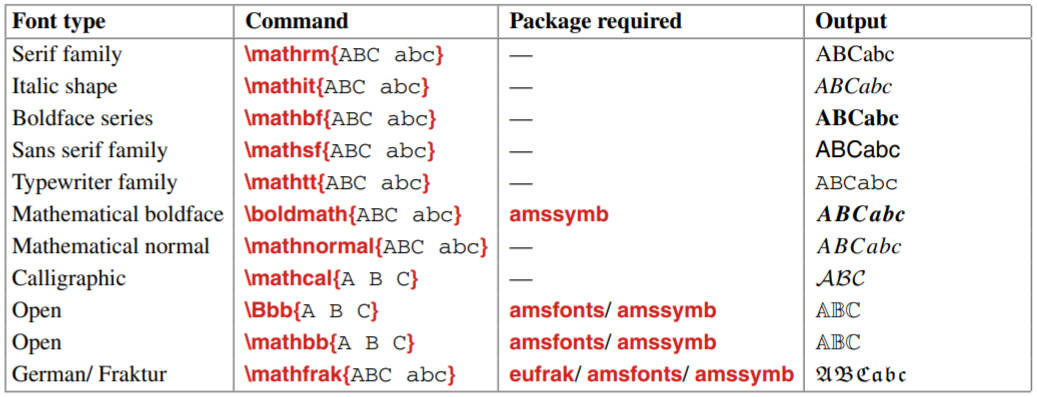
\includegraphics[height=4.5cm]{Math Fonts.png}
    \end{figure}
\end{frame}

\begin{frame}{Особенности типографии: тире и дефис}
    \begin{itemize}
        \item дефисы в~словах: из-за $\delta$-функции
            \linline{дефисы в~словах: из-за $\delta$-функции}

        \item диапазоны чисел: страницы~3--7
            \linline{диапазоны чисел: страницы~3--7}

        \item тире в~предложениях: Это~--- тире.
            \linline{тире в~предложениях: Это~--- тире.}

        \item минусы в~формулах: $-f(-x)=f(x)$
            \linline{минусы в~формулах: $-f(-x)=f(x)$}
    \end{itemize}
\end{frame}

\begin{frame}{Особенности типографии: кавычки}
    \begin{itemize}
        \item Французские <<ёлочки>>

        \linline{Французские <<ёлочки>>}

        \item Немецкие ,,лапки или 99--66‘‘

        \linline{Немецкие ,,лапки или 99--66‘‘}

        \item Английские ‘‘лапки или 66--99’’

        \linline{Английские ‘‘лапки или 66--99’’}

        \item Неверно: ,,нигде так не принято’’

        \linline{Неверно: ,,нигде так не принято’’}

        \item Неверно: ’’и так тоже никто не делает‘‘

        \linline{Неверно: ’’и так тоже никто не делает‘‘}

        \item Неверно: "а это вообще не кавычки"

        \linline{Неверно: "а это вообще не кавычки"}
    \end{itemize}
\end{frame}

\begin{frame}[fragile]{Список литературы}
\begin{lcode}
Ссылка в тексте на публикацию~\cite{vorontsovLX}.
\end{lcode}

\begin{lcode}
% В конце документа
\section{Список литературы}
\begin{thebibliography}{99}
    \bibitem{vorontsovUrl}
    Воронцов К. В., Полезная информация для
    пользователей \LaTeX,
    \url{www.ccas.ru/voron/latex.html}

    \bibitem{vorontsovLX}
    Воронцов К. В., \LaTeX в примерах, 2005,
    \url{www.ccas.ru/voron/download/voron05latex.pdf}
\end{thebibliography}
\end{lcode}
\end{frame}

\begin{frame}[fragile]{Список литературы}
\begin{lcode}
Ссылка в тексте на публикацию~\cite{blei06variational}.
% В конце документа
\section{Список литературы}
\bibliographystyle{gost71s}
\bibliography{references}
\end{lcode}

В файле \texttt{references.bib}:
\begin{lcode}
 @ARTICLE{blei06variational,
  author =       {D. Blei and M. Jordan},
  title =        {Variational inference...},
  journal =      {Journal of Bayesian Analysis},
  year =         {2006},
  pages =        {121--144},
}
\end{lcode}
\end{frame}

\section{LaTeX и русский язык}
\subsection*{}

\begin{frame}[fragile]\frametitle{BibTeX и русский язык}
BibTex не дружит с кириллицей и utf-8 одновременно!

\hfill

\textbf{Способ 1. } Сохранить файл с библиографией в кодировке \texttt{cp1251}, при запуске предупредить о ней

(либо вы счастливый обладатель Windows)

\hfill

\begin{lcode}
\inputencoding{cp1251}
\bibliographystyle{gost71s}
\bibliography{references_rus_cp1251}
\end{lcode}

\hfill

\end{frame}

\begin{frame}[fragile]\frametitle{BibTeX и русский язык}
BibTex не дружит с кириллицей и utf-8 одновременно!

\hfill

\textbf{Способ 2. } Использовать при компиляции \texttt{bibtexu} вместо \texttt{bibtex}

(если вы несчастный обладатель Linux)
\end{frame}

\begin{frame}[fragile]\frametitle{BibTeX и русский язык}
    BibTex не дружит с кириллицей и utf-8 одновременно!

    \hfill

    \textbf{Способ 3. } Использовать библиотеку \texttt{biblatex}

\begin{lcode}
% В преамбуле подключаем библиотеку
\usepackage[bibstyle=gost-numeric]{biblatex}
% В преамбуле указываем файл с библиографией
\addbibresource{references_rus_utf8.bib}
% Цитируем статью
\cite{russianarticle}
% Выводим список процитированных документов
\printbibliography
\end{lcode}
\end{frame}

\begin{frame}[fragile]\frametitle{BibTeX и русский язык}
    Для того, чтобы документ появился в списке литературы его необходимо процитировать в тексте~\cite{russianarticle},~\cite{bar2001fast}

    \printbibliography
\end{frame}

\begin{frame}[fragile]\frametitle{Русский язык в списках}

Переопределить счётчики списков второго уровня на русские буквы:

\begin{lcode}
\renewcommand{\theenumii}{\asbuk{enumii}}
\end{lcode}

    \hfill

    \renewcommand{\theenumii}{\asbuk{enumii}}

    \begin{enumerate}
        \item внешний элемент списка;
        \item другой внешний элемент;
            \begin{enumerate}
                \item внутренний элемент 1
                \item внутренний элемент 2
                \item внутренний элемент 3
            \end{enumerate}
    \end{enumerate}

\end{frame}

\section{Подсветка кода}
\subsection*{}

\begin{frame}[fragile]\frametitle{\texttt{verbatim}}
Окружение \linline{verbatim} ---  запрещает LaTeX обрабатывать вставленный текст, отображает код как есть

\begin{lcode}
\begin{verbatim}
def sum(list_of_numbers):
my_sum = 0
for elem in list_of_numbers:
my_sum += elem
return my_sum
\end{verbatim}
\end{lcode}

\begin{verbatim}
def sum(list_of_numbers):
my_sum = 0
for elem in list_of_numbers:
my_sum += elem
return my_sum
\end{verbatim}

\end{frame}

\begin{frame}[fragile]\frametitle{Пакет \texttt{listings}}
Пакет \linline{listings} ---  мощный пакет LaTeX, позволяющий настраивать специфическое оформление для кода

\begin{lcode}
\begin{lstlisting}
def sum(list_of_numbers):
my_sum = 0
...
\end{lstlisting}
\end{lcode}

\begin{lstlisting}
def sum(list_of_numbers):
my_sum = 0
for elem in list_of_numbers:
my_sum += elem
return my_sum
\end{lstlisting}

\hfill

Правда, по умолчанию он будет работать почти как \linline{verbatim}...
\end{frame}


\begin{frame}[fragile]\frametitle{Пакет \texttt{listings}}
\begin{minted}[fontsize=\small]{latex}
\usepackage{listings}
\usepackage{color}

\lstdefinestyle{myLatexStyle}{
    basicstyle=\small\ttfamily,
    language={python},
    numbersep=5mm, numbers=left, numberstyle=\tiny,
    breaklines=true,frame=single,framexleftmargin=8mm,
    xleftmargin=8mm, backgroundcolor=\color{green!5},
    frameround=fttt,escapeinside=??, rulecolor=\color{red},
    morekeywords={reduce},
    keywordstyle=\color[rgb]{0,0,1},
    commentstyle=\color[rgb]{0.133,0.545,0.133},
    stringstyle=\color[rgb]{0.627,0.126,0.941}
}
\lstset{style=myLatexStyle}
\end{minted}

\end{frame}

\begin{frame}[fragile]\frametitle{Пакет \texttt{minted}}
Пакет \linline{minted} ---  пакет \LaTeX, позволяющий настраивать оформление кода

\hfill

Плюс \linline{minted} --- большое число предустановленных тем

\begin{lcode}
\begin{minted}[fontsize=\small]{python}
def sum(list_of_numbers):
my_sum = 0
...
\end{minted}
\end{lcode}

\begin{minted}[fontsize=\small]{python}
def sum(list_of_numbers):
my_sum = 0
for elem in list_of_numbers:
my_sum += elem
return my_sum
\end{minted}

\end{frame}

\begin{frame}[fragile]\frametitle{Пакет \texttt{minted}}
\begin{lcode}
Команда \mintinline{latex}{\mintinline{language}{}}
для оформления кода внутри связного текста.
Например, С++:
\mintinline{C++}{std::vector<int> b{1, 2, 3};}
\end{lcode}

\hfill

Команда \linline{\mintinline{language}{}} для оформления кода внутри связного текста. Например, С++: \mintinline{C++}{std::vector<int> b{1, 2, 3};}

\end{frame}

\begin{frame}[fragile]\frametitle{Плюсы и минусы различных способов}
    \begin{itemize}
        \item \linline{verbatim}
            \begin{itemize}
                \item[+] Быстро, не требует настройки
                \item[--] Отсутствие возможностей настройки
            \end{itemize}
        \item \linline{lstlisting}
            \begin{itemize}
                \item[+] Огромное количество возможностей
                \item[--] Красивый результат требует тщательной настройки
                \item[--] Сложно задавать свои окружения для разных языков
            \end{itemize}
        \item \linline{minted}
            \begin{itemize}
                \item[+] Огромное количество возможностей
                \item[+] Больше число предустановленных тем
                \item[+] Легко задавать окружения для разных языков
                \item[--] Есть проблемы при установке
            \end{itemize}
    \end{itemize}
\hfill

При использовании всех этих пакетов объявление слайда приходится записывать так:
\begin{minted}[fontsize=\small]{latex}
\begin{frame}[fragile]\frametitle{Плюсы и минусы
различных способов}
\end{minted}
\end{frame}

\section{TikZ и PFG}
\subsection*{}
\begin{frame}[fragile]\frametitle{\texttt{TikZ} и \texttt{PFG}}
\texttt{PFG} --- низкоуровневый пакет для векторной графики в \TeX

\hfill

\texttt{TikZ} --- высокоуровневое расширение этого пакета

\hfill

\href{http://www.texample.net/tikz/}{http://www.texample.net/tikz/} --- сайт с примерами работы

\hfill

\href{http://www.texample.net/tikz/}{http://www.texample.net/tikz/} --- сайт с примерами работы

\hfill

Самое подробное~руководство доступно по \href{http://www.texample.net/media/pgf/builds/pgfmanualCVS2012-11-04.pdf}{ссылке}.

\end{frame}

\begin{frame}[fragile]\frametitle{Изображение графиков}
\begin{minipage}{0.49\linewidth}
    \begin{tikzpicture}[scale=0.6]
        \begin{axis}[
            %title = Функции пороговой обработки,
            line width = 1pt,
            xlabel = {$x$},
            xtick={-1, 0, 1},
            xticklabels={-T, 0, T},
            ytick={-1, 0, 1},
            yticklabels={-T, 0, T},
            mark=none,
            legend entries={hard, soft, hybrid},
            legend style={legend pos=south east, font=\Large}
        ]
        \addplot[blue] coordinates {(-2, -2) (-1, -1) (-1, 0) (1, 0) (1, 1) (2, 2)};
        \addplot[red] coordinates {(-2, -1) (-1, 0) (1, 0) (2, 1)};
        \addplot[green, domain=-2:-1] {x - 1/x};
        \addplot[green, domain=1:2] {x - 1/x};
        \addplot[green, domain=-1:1] {0};
        \addplot[blue, dashed] coordinates {(-2, -2) (2, 2)};
        \end{axis}
    \end{tikzpicture}
\end{minipage}
\begin{minipage}{0.49\linewidth}
\begin{minted}[fontsize=\small]{latex}
\begin{tikzpicture }[scale=0.7]
    \begin{axis}[
        line width = 1pt,
        xlabel = {$x$},
        xtick={-1, 0, 1},
        xticklabels={-T, 0, T},
        ytick={-1, 0, 1},
        yticklabels={-T, 0, T},
        mark=none,
        legend entries={
            hard, soft, hybrid
        },
        legend style={
            font=\Large,
            legend pos=south east
        }
    ]
    ...
\end{minted}
\end{minipage}
\end{frame}

\begin{frame}[fragile]\frametitle{Изображение графиков}
\begin{minipage}{0.49\linewidth}
    \begin{tikzpicture}[scale=0.6]
        \begin{axis}[
            %title = Функции пороговой обработки,
            line width = 1pt,
            xlabel = {$x$},
            xtick={-1, 0, 1},
            xticklabels={-T, 0, T},
            ytick={-1, 0, 1},
            yticklabels={-T, 0, T},
            mark=none,
            legend entries={hard, soft, hybrid},
            legend style={legend pos=south east, font=\Large}
        ]
        \addplot[blue] coordinates {
            (-2, -2) (-1, -1) (-1, 0)
            (1, 0) (1, 1) (2, 2)
        };
        \addplot[red] coordinates {(-2, -1) (-1, 0) (1, 0) (2, 1)};
        \addplot[green, domain=-2:-1] {x - 1/x};
        \addplot[green, domain=1:2] {x - 1/x};
        \addplot[green, domain=-1:1] {0};
        \addplot[blue, dashed] coordinates {(-2, -2) (2, 2)};
        \end{axis}
    \end{tikzpicture}
\end{minipage}
\begin{minipage}{0.49\linewidth}
\begin{minted}[fontsize=\small]{latex}
    ...
    \addplot[blue] coordinates {
        (-2, -2) (-1, -1) (-1, 0)
        (1, 0) (1, 1) (2, 2)
    };
    \addplot[blue, dashed]
    coordinates {(-2, -2) (2, 2)};
    \addplot[red] coordinates ...
    \addplot[green, domain=-2:-1]
    {x - 1/x};
    \addplot[green, domain=1:2]
    {x - 1/x};
    \addplot[green, domain=-1:1]
    {0};
    \end{axis}
\end{tikzpicture}
\end{minted}
\end{minipage}

\end{frame}

\begin{frame}[fragile]\frametitle{Изображение линий уровня}
\bigskip
Линии уровня для $\Vert X\vec w-\vec y\Vert_2$ и области $\|w\|_1 \leqslant \kappa, \|w\|_2 \leqslant \kappa$:

\begin{minipage}{0.49\linewidth}
\[
    \begin{tikzpicture}
        \draw[->] (-1.5, 0) -- (3, 0) node[anchor=north] {$x_1$};
        \draw[->] (0, -1.5) -- (0, 3.5) node[anchor=east] {$x_2$};
        \draw (-0.2, -0.2) node[scale=0.8] {$0$};
        \draw (2, 3.5 ) node {$l_1$-регуляризация};

        \draw[blue] (0.83, 2) circle (1.2cm);
        \draw[blue] (0.83, 2) circle (0.9cm);
        \draw[blue] (0.83, 2) circle (0.6cm);
        \draw[blue] (0.83, 2) circle (0.3cm);

        \draw[red] (0, -1.1) -- (1.1, 0) -- (0, 1.1) -- (-1.1, 0) -- (0, -1.1);
        \filldraw[pattern color=red, pattern=north west lines] (0, -1.1) -- (1.1, 0) -- (0, 1.1) -- (-1.1, 0) -- (0, -1.1);
        %\draw[red] (0, -0.83) -- (0.83, 0) -- (0, 0.83) -- (-0.83, 0) -- (0, -0.83);
        %\draw[red] (0, -0.5) -- (0.5, 0) -- (0, 0.5) -- (-0.5, 0) -- (0, -0.5);

        \node at (0, 1.1) [scale=0.4,shape=circle,draw=blue,fill=blue] {};
        \draw (-0.1, 2) -- (0.1, 2);
        \draw (-0.2, 1.9) node[scale=0.8] {$y_2$};
        \draw (0.83, -0.1) -- (0.83, 0.1);
        \draw (0.83 + 0.1, -0.2) node[scale=0.8] {$y_1$};
    \end{tikzpicture}
\]
\end{minipage}
\begin{minipage}{0.49\linewidth}
\[
    \begin{tikzpicture}
        \draw[->] (-1.5 + 8, 0) -- (3 + 8, 0) node[anchor=north] {$x_1$};
        \draw[->] (0 + 8, -1.5) -- (0 + 8, 3.5) node[anchor=east] {$x_2$};
        \draw (-0.2 + 8, -0.2) node[scale=0.8] {$0$};
        \draw (3.5 + 6.5, 3.5 + 0.2) node {$l_2$-регуляризация};

        \draw[blue] (0.83 + 8, 2) circle (1.2cm);
        \draw[blue] (0.83 + 8, 2) circle (0.9cm);
        \draw[blue] (0.83 + 8, 2) circle (0.6cm);
        \draw[blue] (0.83 + 8, 2) circle (0.3cm);

        \draw[red] (0.0 + 8, 0) circle (0.94cm);
        \filldraw[pattern color=red, pattern=north west lines] (0.0 + 8, 0) circle (0.94cm);
        %\draw[red] (0.0 + 8, 0) circle (0.65cm);
        %\draw[red] (0.0 + 8, 0) circle (0.4cm);

        \node at (0.3 + 8, 0.9) [scale=0.4,shape=circle,draw=blue,fill=blue] {};
        \draw (-0.1 + 8, 2) -- (0.1 + 8, 2); % засечка на оси
        \draw (-0.2 + 8, 1.9) node[scale=0.8] {$y_2$};
        \draw (0.83 + 8, -0.1) -- (0.83 + 8, 0.1);
        \draw (0.83 + 0.1 + 8, -0.2) node[scale=0.8] {$y_1$};
    \end{tikzpicture}
\]
\end{minipage}
\end{frame}

\begin{frame}[fragile]\frametitle{Изображение линий уровня}
\begin{minted}[fontsize=\small]{latex}
\begin{tikzpicture}
    \draw[->] (-1.5, 0) -- (3, 0) node[anchor=north] {$x_1$};
    \draw[->] (0, -1.5) -- (0, 3.5) node[anchor=east] {$x_2$};
    \draw (-0.2, -0.2) node[scale=0.8] {$0$};
    \draw (2, 3.5 ) node {$l_1$-регуляризация};

    \draw[blue] (0.83, 2) circle (1.2cm);
    \draw[blue] (0.83, 2) circle (0.9cm);
    \draw[blue] (0.83, 2) circle (0.6cm);
    \draw[blue] (0.83, 2) circle (0.3cm);

    \draw[red] (0, -1.1) -- (1.1, 0) -- (0, 1.1) --
    (-1.1, 0) -- (0, -1.1);
    \filldraw[pattern color=red, pattern=north west lines]
    (0, -1.1) -- (1.1, 0) -- (0, 1.1) --
    (-1.1, 0) -- (0, -1.1);
    ...
\end{minted}
\end{frame}

\begin{frame}[fragile]\frametitle{Изображение графа}
\begin{minipage}{0.45\linewidth}
    \begin{tikzpicture}[scale=2]
        \node (p1) at (0,0) [scale=0.6,shape=circle,draw=black,fill=white] {1};
        \node (p2) at (2,0) [scale=0.6,shape=circle,draw=black,fill=yellow] {2};
        \node (p3) at (1,1) [scale=0.6,shape=circle,draw=red,fill=white] {3};
        \node (p4) at (2,2) [scale=0.6,shape=rectangle,draw=black,fill=white] {4};
        \node (p5) at (0,2) [scale=0.6,shape=circle,draw=black,fill=white] {5};
        \node (p6) at (1,2) [scale=0.6,shape=circle,draw=black,fill=white] {6};

        \draw (p1) -- (p3) -- (p5);
        \draw (p2) -- (p3) -- (p4);
        \draw[->] (p6) -- (p3);
    \end{tikzpicture}
\end{minipage}
\begin{minipage}{0.54\linewidth}
\begin{minted}[fontsize=\small]{latex}
\begin{tikzpicture }[scale=2]
    \node (p1) at (0,0) [
        scale=0.6,shape=circle,
        draw=black,fill=white
    ] {1};
    \node (p2) at (2,0) [
        scale=0.6, shape=circle,
        draw=black, fill=yellow
    ] {2};
    \node (p3) at (1,1) [
        scale=0.6, shape=circle,
        draw=red, fill=white
    ] {3};
    \node (p4) at (2,2) [
        scale=0.6, shape=rectangle,
        draw=black, fill=white
    ] {4};
    ...
\end{minted}
\end{minipage}

\end{frame}

\begin{frame}[fragile]\frametitle{Изображение графа}

\begin{minipage}{0.45\linewidth}
    \begin{tikzpicture}[scale=2]
        \node (p1) at (0,0) [scale=0.6,shape=circle,draw=black,fill=white] {1};
        \node (p2) at (2,0) [scale=0.6,shape=circle,draw=black,fill=yellow] {2};
        \node (p3) at (1,1) [scale=0.6,shape=circle,draw=red,fill=white] {3};
        \node (p4) at (2,2) [scale=0.6,shape=rectangle,draw=black,fill=white] {4};
        \node (p5) at (0,2) [scale=0.6,shape=circle,draw=black,fill=white] {5};
        \node (p6) at (1,2) [scale=0.6,shape=circle,draw=black,fill=white] {6};

        \draw (p1) -- (p3) -- (p5);
        \draw (p2) -- (p3) -- (p4);
        \draw[->] (p6) -- (p3);
    \end{tikzpicture}
\end{minipage}
\begin{minipage}{0.54\linewidth}
\begin{minted}[fontsize=\small]{latex}
    ...
    \node (p5) at (0,2) [
        scale=0.6, shape=circle,
        draw=black, fill=white
    ] {5};
    \node (p6) at (1,2) [
        scale=0.6, shape=circle,
        draw=black, fill=white
    ] {6};

    \draw (p1) -- (p3) -- (p5);
    \draw (p2) -- (p3) -- (p4);
    \draw[->] (p6) -- (p3);
\end{minted}
\end{minipage}

\end{frame}

\begin{frame}[fragile]\frametitle{Сохранение графиков экспериментов}
Проблема: провели эксперимент, сохранили график, но...
    \begin{center}
        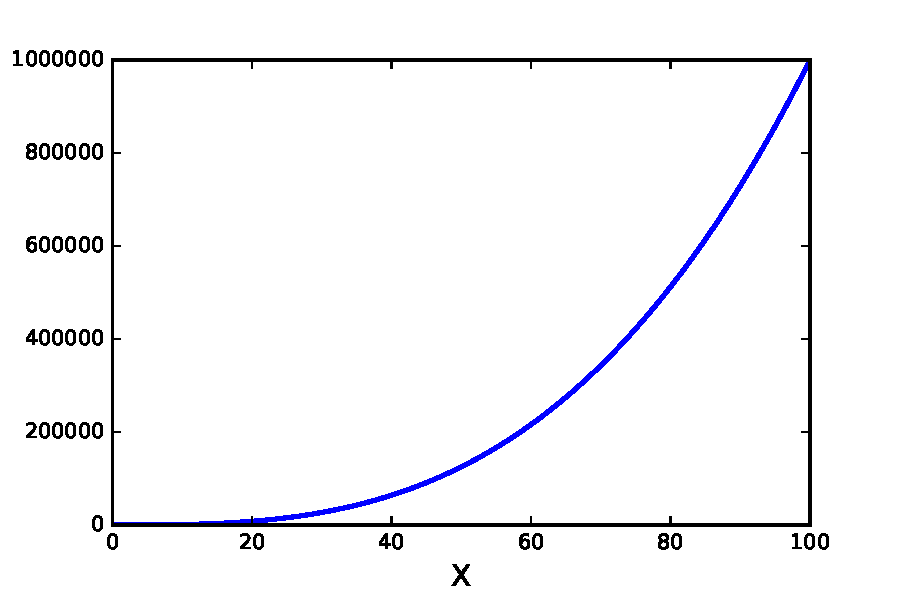
\includegraphics[scale=0.4]{tmp_fig.pdf}
    \end{center}

    забыли подписать ось $y$.
\end{frame}

\begin{frame}[fragile]\frametitle{Интеграция \texttt{Python} и \texttt{TikZ}}
Пакет \pinline{matplotlib2tikz} позволяет сохранять графики в формате \linline{TikZ}.

\hfill

\begin{pcode}
import matplotlib.pyplot as plt
from matplotlib2tikz import save as tikz_save

x = [i for i in range(0, 101, 1)]
y = [x_el ** 3 for x_el in x]

plt.plot(x, y, linewidth=2)
plt.xlabel('X', fontsize=14)

tikz_save('tmp_tikz.txt')
\end{pcode}
\end{frame}

\begin{frame}[fragile]\frametitle{Результат сохранения картинки}
\begin{lcode}
% This file was created by matplotlib2tikz v0.6.13.
\begin{tikzpicture }
\begin{axis}[
xlabel={X},
xmin=0, xmax=100,
ymin=0, ymax=1000000,
axis on top,
tick pos=both
]
\addplot [thick, blue, forget plot]
table {%
0 0
1 1
2 8
...
\end{lcode}
\end{frame}

\begin{frame}[fragile]\frametitle{Вставка картинки в формате \texttt{.tikz}}

\begin{minipage}{0.49\linewidth}
\begin{minted}[]{latex}
\newlength\figureheight
\newlength\figurewidth
\setlength\figureheight{6cm}
\setlength\figurewidth{6cm}
\input{tmp_tikz.txt}
\end{minted}
\end{minipage}
\begin{minipage}{0.49\linewidth}
    \newlength\figureheight
    \newlength\figurewidth
    \setlength\figureheight{6cm}
    \setlength\figurewidth{6cm}
    \input{Figures/tmp_tikz.txt}
\end{minipage}

\hfill

Что это нам даёт?
\end{frame}

\begin{frame}[fragile]\frametitle{Вставка картинки в формате \texttt{.tikz}}
Картинка сохранена в удобном текстовом представлении

\hfill

Добавим название оси $y$ отредактировав текстовый файл:

\hfill

\begin{minipage}{0.49\linewidth}
\begin{verbatim}
...
\begin{axis}[
xlabel={X},
ylabel={Y},
...
\end{verbatim}
\end{minipage}
\begin{minipage}{0.49\linewidth}
    \setlength\figureheight{5cm}
    \setlength\figurewidth{5cm}
    \input{Figures/tmp_tikz2.txt}
\end{minipage}
\end{frame}

\begin{frame}{Полезные ссылки}
\begin{thebibliography}{}
    %Нарисовать текущий элемент в стиле online-ссылки
    \setbeamertemplate{bibliography item}[online]
    \bibitem{lvovsky}
    Львовский~С.\,М. Набор и вёрстка в системе \LaTeX. 2003.
    \url{http://www.ptep-online.com/ctan/llang2003.pdf}

    \setbeamertemplate{bibliography item}[online]
    \bibitem{vorontsovLatex}
    Воронцов К. В. \LaTeX\ в примерах, 2005,
    \url{http://www.ccas.ru/voron/download/voron05latex.pdf}

    \bibitem{voronstovhints}
    Написание отчётов и статей (рекомендации),
    \href{www.machinelearning.ru/wiki/index.php?title=Категория:Рекомендации_для_студентов}{ссылка}.

    \bibitem{baldin}
    Балдин Е.М. LATEX, GNU/Linux и русский стиль,
    \href{http://www.apmath.spbu.ru/cnsa/tex/BaldinEM_LaTEX_v_Rossii.pdf}{ссылка}.

    \bibitem{latex_24}
    Dilip Datta. LaTeX in 24 Hours,
    \href{http://www.tezu.ernet.in/dmech/people/ddatta_files/attachment/LaTeX_24H_Note.pdf}{ссылка}.

    \bibitem{cheatlist}
    Шпаргалка по частоиспользуемым математическим символам в \LaTeX,
    \href{https://www.caam.rice.edu/~heinken/latex/symbols.pdf}{ссылка}.
\end{thebibliography}
\end{frame}

\end{document}
